\documentclass{scu-thesis}
 \usepackage{graphicx}	% for including graphics
 \usepackage{amsmath}	% for advanced typesetting of mathematics
 \usepackage{txfonts}	% for using the Times-Roman font
 \usepackage{natbib}	% for better citation styles
 \usepackage{hyperref}
 \usepackage[font=small,format=plain,labelfont=bf,up,textfont=it,up]{caption}%styalize captions
 \usepackage{cleveref}%references
\usepackage{paralist}% for compact item


% These must be set first ... the rest of the thesis commands rely on them.

\author{Cris Madrigal}
\author{Jiachi Zhang}
\author{Nicholas Peacock}
\author{Brogan O'Hara}
\title{RSL Autonomous Rover}
\department{Department of Electrical Engineering}
\department{Department of Computer Engineering}
\department{Department of Mechanical Engineering}
\degree{Bachelor of Science in Electrical Engineering}
\degree{Bachelor of Science in Computer Science and Engineering}
\degree{Bachelor of Science in Mechanical Engineering}


% Only bachelor's theses should have multiple authors and/or be from
% multiple departments.  Signatures required:
%
% Bachelor's theses: advisor(s), department chair(s)
% Master's theses: advisor, reader, department chair
% Doctoral theses: doctoral committee (including advisor), department chair

\begin{document}
\frontmatter
\signature{Thesis Advisor}
\signature{Department Chair}
\signature{Department Chair}
\signature{Department Chair}

\maketitle
%\begin{abstract}
A good abstract is a concise summary (1--2 paragraphs) of the entire
project: introduction, problem statement, work accomplished, results,
conclusions, and recommendations. When you write the abstract, imagine
that the reader will not read anything else, but that you must get
your major point across immediately. This requires efficiency of words
and phrases. An abstract is written to stand alone, without jargon or
reference to figures and tables in the report body.
\end{abstract}


\tableofcontents
\listoffigures

\mainmatter
\chapter{Introduction}

The advancement of technology has allowed humans to venture into worlds that 10 years ago would not have even been possible.  Increased processing power allows for the creation of more complex control algorithms to manage our evolving systems.  These control algorithms may be used in a variety of applications and most notably, in the development of autonomous features in vehicles.  All vehicles currently have some sort of driver assist function installed: cruise control, anti-locking brakes, and etc.  These are pieces of technology that did not exist ten years ago, but now we take them for granted.  However, imagine a world where everyone has a vehicle that can reach a destination with minimal human interaction and input.  The driver would be able to sit back, relax, and use the driving time to be more enjoyable.  The average American spends approximately 87 minutes behind the wheel each day.\cite{abcnews} TThis is time that could be used for more productive or enjoyable tasks.  Autonomous cars will lead to less congestion on our roadways and fewer accidents.  Although many like to think that they are good drivers, statistics show that human error is the cause for around 85\% of all accidents. \cite{aa1car} These accidents are usually caused by the driver getting distracted, not adjusting properly to driving conditions or consuming narcotics.  We have control over these issues but lack the discipline to do so. Eliminating these human errors and continuing the advancement of technology in our vehicles leads to an improvement of life by minimizing the risk of driving.  The dream of a fully autonomous vehicle is soon to become a reality.  

In 2004, the Defense Advanced Research Projects Agency (DARPA) presented a challenge to create an autonomous vehicle with the ability to navigate to different waypoints in a preset course.  The challenge was at first unsuccessful, as nobody was able to create a vehicle that was able to navigate the entire course.  But in 2005, five teams were able to complete the 130 mile course.  After only one year, there was a significant amount of progress in the field of vehicle autonomy.  Imagine what could happen in five.  Four states currently have laws that allow for the testing of autonomous vehicles and this number is expected to grow as the technology improves.  Google is leading the charge.  Their team is headed by 15 engineers, who were people that competed in the DARPA challenge in 2005.  Their most recent prototype has no steering wheel or pedals installed; it essentially eliminates the driver?s ability to override the vehicle?s controls.  This prototype currently has some limitations, however. It cannot be driven in heavy rain or snow, as those weather conditions interfere with the sensors, and it also has difficulty distinguishing and avoiding potholes and other objects.  Google hopes to have all of these issues fixed by 2020 so that they can manufacture vehicles that can be used in all conditions.  

The motivation behind our project is to use emerging technology in an educational manner to improve the lives of others.  Future students and researches will be able to build upon what we have accomplished and make strides to improve this new technology.

\section{Literature Review}

{\bf Coming Soon}

\section{Problem Statement}

The objective of the RSL Rover is to use the existing drive-by-wire control system and interface for operating an all-terrain vehicle to build an autonomous system for the detection of underground objects, such as landmines. The tasks for the project are three-fold:\\
\begin{compactitem}
\item Implement controllers that will interface with the current system, allowing the rover to be given an objective and independently navigate to complete the task.
\item Install sensors on the vehicle and develop an algorithm to enhance autonomous driving, and detect underground objects for a variety of applications. 
\item Develop an effective safety mechanism and emergency shutoff method that will prevent the rover from causing injury and damage.
\end{compactitem}
The result of this project is a highly capable autonomous vehicle that may be used in a variety of capacities, including the detection of landmines, underground pipes, and etc, to serve areas that face these obstacles.

\section{Vehicle Background}

This vehicle was originally built to compete in the 2004 \& 2005 DARPA challenge by Team Overbot.  It failed to qualify for the national competition both years and was eventually donated to a local university where it was used for educational purposes.  When the team last year obtained the vehicle, all of the internal components were a mess.  They were able to revert most of the changes over the years to set it back to factory standards.  On top of that they ``...built a hierarchical control system, robust actuator mounts, and an effective safety system? \cite{UnmannedAerialAndGround} in a flexible manner that will allow for upgrades in the future. With these additions they were able to control the vehicle remotely. \Cref{roverSide,,roverFront,,roverOver} show the existing vehicle.

\begin{figure}[h!]
\begin{center}
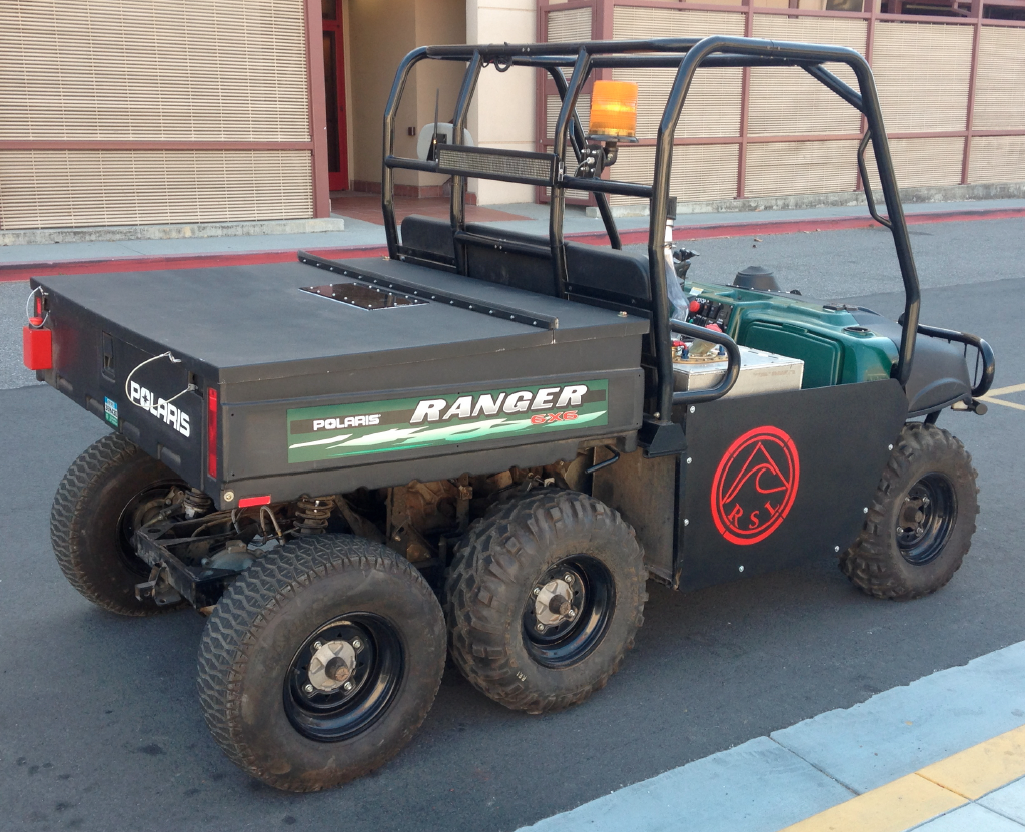
\includegraphics[width=.8\textwidth]{Figures/RSLRover_SideVeiw.png}
\caption{RSL Rover Side View}
\label{roverSide}
\end{center}
\end{figure}

\begin{figure}[h!]
\begin{center}
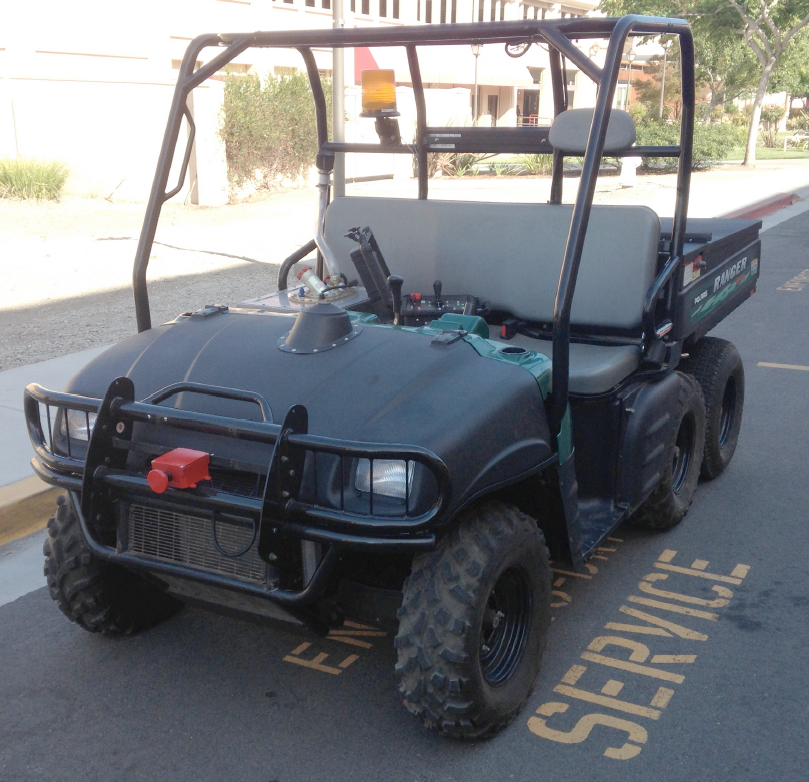
\includegraphics[width=.8\textwidth]{Figures/Rover_Front.png}
\caption{RSL Rover Front View}
\label{roverFront}
\end{center}
\end{figure}

\begin{figure}[h!]
\begin{center}
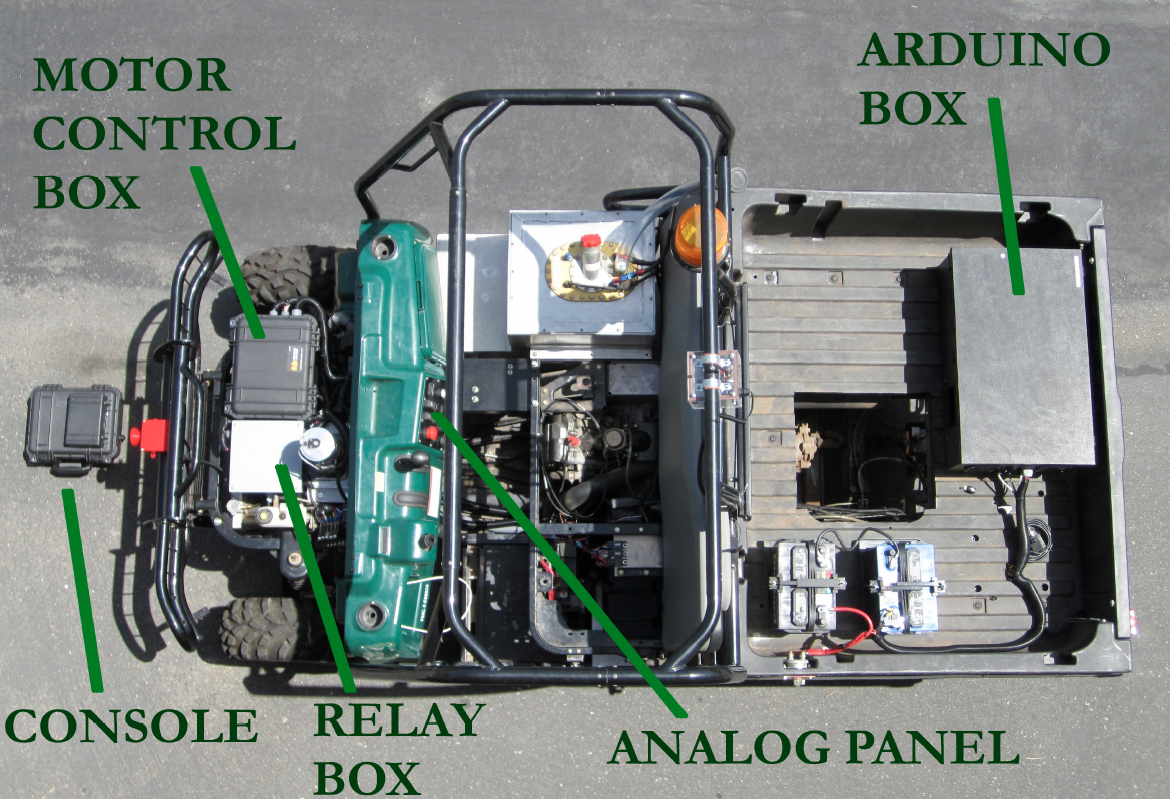
\includegraphics[width=.8\textwidth]{Figures/Rover_Overhead.png}
\caption{RSL Rover Overhead View}
\label{roverOver}
\end{center}
\end{figure}













\chapter{System-Level Design}

	\section{Overview}
	
	The mission architecture of the system is shown in \Cref{SLsketch}. 
\begin{figure}[h!]
\begin{center}
%\includegraphics[width=\textwidth]{Figures/.png}
\caption[System Level Sketch]{Shown is system level sketch, or mission architecture.}
\label{SLsketch}
\end{center}
\end{figure}	
This diagram shows the overall goal of the project. The vehicle traverses a field by following a path and avoiding any objects that may be in its way.  This will be done with the sensors that are attached to the vehicle, as shown.  Information about the status of the sensors, the speed and the vehicle?s performance will be relayed to the on-board microprocessors (Edison).  This information will then be saved and input into an autopilot navigation system and obstacle avoidance control algorithm.  Multiple Edison microprocessor boards will be necessary so that we do not have any issues with data processing and backlogging.  The information saved on the processor will be downloadable as a .txt file to be viewed by the user.  This makes troubleshooting easier.  A simple breakdown of this process is shown in \Cref{Block}.
\begin{figure}[h!]
\begin{center}
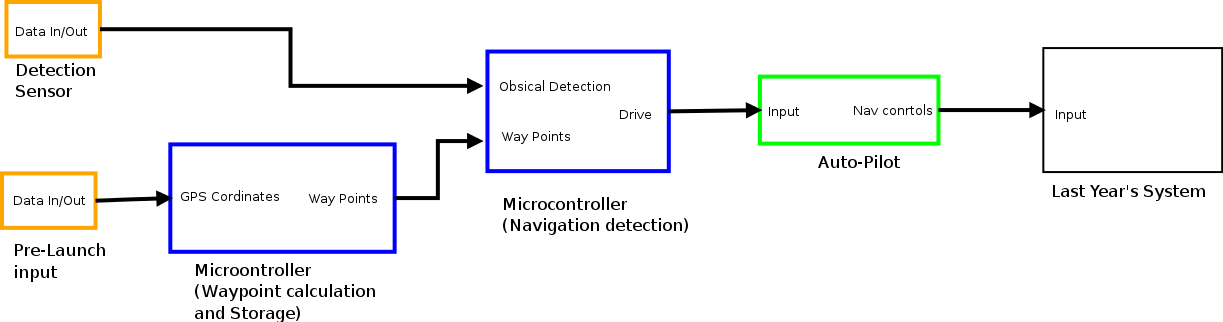
\includegraphics[width=\textwidth]{Figures/RSL_Rover_BlockDiagram.png}
\caption[Component Block Diagram]{Shown is a simplified component block diagram showing general signal flow. It abstracts away all of the previous years system into a single block on diagram because all work is to be done upstream of their work.}
\label{Block}
\end{center}
\end{figure}
The vehicle will be able to make a decision to change course in a minimal amount of time.  Our additions to the vehicle will be able to interface with the previous system.  Our Edison processors will interact with the Arduino microcontrollers currently on the board to control the vehicle?s actuators. \Cref{oldBlock} is the previous years simplified block diagram, and this will help give a general understanding of the entire system.
\begin{figure}[h!]
\begin{center}
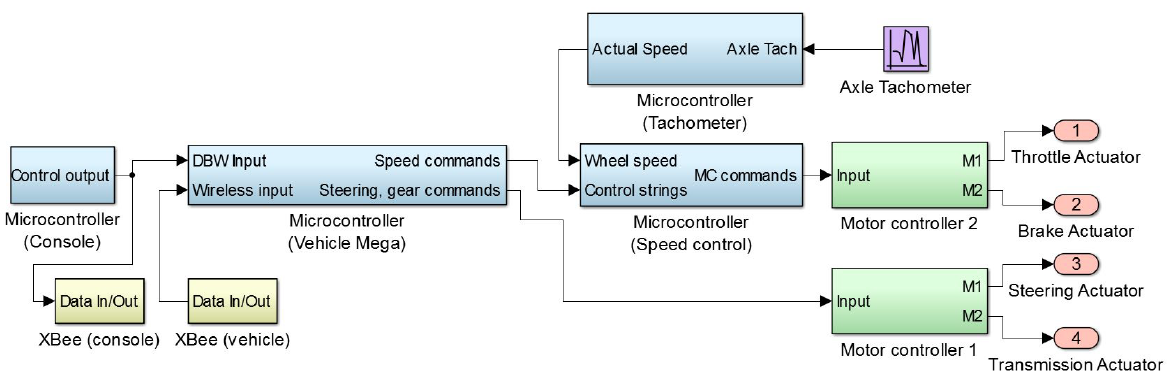
\includegraphics[width=\textwidth]{Figures/PreviousCBD.png}
\caption[Previous Year's Component Block Diagram]{Simplified block diagram of previous work.}
\label{oldBlock}
\end{center}
\end{figure}


\section{Customer Definition and Needs}
The objective of this project is to retrofit the current unmanned land vehicle with sensors and microprocessors to allow the vehicle to have autonomous capabilities.  The process of doing so should be well documented and the final product should be easy to use.  This is necessary so that future students may use the vehicle with a relatively small learning curve.  The vehicle has some built in constraints that are not fixable. These include: the weight, size, engine power, etc.  However, the vehicle is still relatively flexible.  Our team will be able to customize the type of sensors we use and determine the user interface, the vehicle speed, accuracy, robustness, and cost to fit in line with the customer needs.

    There are two customers in mind for our project.  The first one is the Robotics Systems Laboratory.  Future undergraduate, graduate and Ph.D. students will be able to use the vehicle to expand their knowledge of control systems, vehicle control, and etc.  Our second customer is a group of farmers in rural locations in California.  Their lack of resources makes it hard for them to compete versus large farming corporations.  We hope that our vehicle will be able to assist them in the detection of underground pipes that may be hidden in their plots of land.  
    
The final product needs to be easy to use and understandable.  Thus, the algorithms used to control the vehicle to be simple and robust enough that users with limited knowledge will not have any issues.   A friendly user interface will allow the user to control aspects of the vehicle without actually having to change the code.  Quality of the parts is also an issue.  We want to retrofit the system with the best parts that our budget allows us; this will decrease the maintenance needed in the future and make it easier for the customer to trust the system.  Also, by using parts manufactured by well-established companies, the components be less likely to become obsolete in the future. 

    Safety is a large concern for us.  Because this system will be autonomous, extra precautions must be taken because a mistake could result in a serious injury or even death. Several safety systems will be implemented to protect both the user and the vehicle.  These include ?dead man? switches that shut off the system if the connection to a sensor is lost, warning signals/sounds from the vehicle, and a maximum speed limit of the vehicle in relation to the environmental conditions and sensor quality.  The safety of the end user is our primary concern.

\section{System Level Requirements}
	The system requirements from the previous year are still valid.  The project will have four focuses:
	
\begin{compactitem}
	\item {\bf Navigation Control:} Vehicle will take in GPS coordinates and use those to traverse a plot of land or path.  When following a predetermined route, the vehicle will not deviate more than 0.5 meters.  A closed loop feedback control system will be implemented to read the feedback and make adjustments if necessary.
	\item {\bf Velocity Control:} The vehicle will try to maintain a 10 mph speed which equates to approximately to 3.6 acres per hour.  The speed can be adjusted depending on the terrain, weather conditions and visibility. The maximum speed will not exceed 13 mph.
	\item {\bf Sensor Control:} Limit the amount of false alarms from the RADAR system to 1\%. This number is a realistic goal due to the type of sensors that we are able to purchase with our funding.   Sensors will be managed by a control algorithm.  The information will be sent to the micro-processors, ideally only one or two sensors per microprocessor to prevent a backup of information.  The latency between the sensor and microprocessor should be less than 500ms.
	\item {\bf Interface/Data Storage:} To make troubleshooting easy, we wish to have the vehicle generate a .txt file every time the vehicle is started to log the vehicle diagnostics and performance, time, GPS, coordinates, activity and status.  
\end{compactitem}

\section{Benchmarking Results}
	{\bf coming soon}

\section{Functional Analysis}
	The project is broken into four major subsystem:
\begin{enumerate}
	\item Navigation
	\item Sensor Interfacing
	\item User Interface
	\item Safety
\end{enumerate}

All of these subsections are intertwined in some way, but it?s easier to understand the work that needs to be done on each one if it is broken down.  This also helps us prioritize which one these we find the most important and how they affect the other subsystems.

The first subsystem, is the Navigation system.  We will be using an off the shelf auto pilot system.  This ArduPilot Mega (APM) comes built in with GPS capabilities and a compass.  The APM will be interfaced with the pre-existing Arduinos that control the actuators.  The information that is being sent to the APM will be interpreted and used to perform the correct actions. 

The second subsystem are how the sensors are going to interface with each other.  We will have several array of sensors in order to limit the amount of false alarms and get the most precise information possible.  The information will be sent to the Edison boards for processing and that information will be relayed to the APM system.

The third subsystem is the user interface.  We want our project to be easy to use for people that do not have a large amount of technical training, so we need to remove any of the unnecessary information that may be presented.  We will be using the open-source software that comes with the APM that allows you to set your customizable programmed course.  We also will allow the users to pull data from the Edison boards after the vehicle has completed its task for system diagnostics.

The fourth subsystem is safety.  This includes hardwires and software automatic shutoffs.  Because the system is autonomous we need to have a way to stop the process from a safe distance if the vehicle malfunctions.  We will also implement code that will shut off the system if any of our sensors are unable to send information to the Edison.  How the wiring is done is also important to safety; it must be made sure that none of those connections will come loose in the driving process.

\section{System Level Issues and Trade-offs}
	
Several issues arose that wasn?t a part of a sub-system but more into the general system level.  We had to decide how much of the old vehicle we wanted to keep and if we wanted to continue to use the same control commands.  These decisions were necessary to make early in order to be able to proceed efficiently on our design.

We inherited this operational drive-by-wire vehicle from last years team.  But we found that the documentation in several cases were incorrect, therefore we had to spend a large amount of time reverse engineering several previous subsystems.  Eventually we were able to get the system functioning as intended.  The reliability of the current vehicle is good enough that we decided we could leave it intact.  The hardware that we are adding to the system will streamlined into the previous work.  We intend to improve the documentation of the vehicle, in both the previous work and our work for this year.

How the vehicle would receive, interpret and respond to motor commands was decided upon by the previous years work.  They developed an algorithm that would specify the steering angle with either a brake or throttle commands.  We wanted to preserve their code as much as possible, so we decided to continue to use their command structure.  The challenge now that we face in getting the external data to translate into the information so that the vehicle can process the commands correctly.  This issue we felt would be easier to solve then changing the entire original system.

	\section{Team and Project Management}

		\subsection{Initial Team Goals}
			Our team is comprised of 3 senior Electrical Engineers and a double major Mechanical/Computer engineer who all have a passion for automotives and exploring different control algorithms.  At the beginning of the year we came up with several goals that we hoped to meet:
			\begin{enumerate}
				\item Improve the original control algorithm if needed, and add any code that may be needed for our portion of the project.
				\item Working with microcontrollers, sensors and safety mechanisms that may be used in the industry.
				\item Find a balance between the project, our school work and our social lives.  We felt this should be a project that we enjoy doing and not turn into a full time job to get it done. 
				\item Obtain a good grade, and have a working prototype done by the end of spring.
			\end{enumerate}
		
		%\subsection{Reflection on Team Goals}
		
\subsection{Mitigating Project Challenges and Working within Constraints}

As with any big project there are a number of issues that arose in the decision making and design of our vehicle.  These major challenges include:

\begin{enumerate}
\item Faulty mechanical equipment
\item Unfamiliar code in regards to the autopilot system and legacy code from previous year
\item Team disagreements
\end{enumerate}

Another challenge that we faced was how to manage our time.  Deciding how the work would be split up and meeting goals that we set for ourselves became an issue due to our lack of experience and manpower.

When these issues arose we were able to come up with creative ways to fix these problems in the most efficient manner, this process included:

\begin{enumerate}
\item Having good communication with one another.  Work that was done will be reported so that the other members would know what issues had either been resolved or needed more work. This way we don?t end up wasting our time doing things that were unnecessary.   It was encouraged to share our opinion and think about possible solutions to the process that we were working on.  This allows us to see the problem from many different angles and possibly choose the best solution.
\item Willingness to seek out help.  Many times we asked others to assist us with issues that we may not be familiar with or to get a second opinion.  Using the resources around us was the best way that we could optimize the way we spent time on a certain portion of the project.
\item Effective documentation.  How the algorithm works, what parts were used, how the wiring is constructed.  Because this is a legacy project we want to leave all the appropriate information organized for next years team.  Having good documentation allows us to quickly refer things when discussing certain matters.
\end{enumerate}
		
		%\subsection{Budget}
		
\subsection{Timeline}
		
When we started in Fall we wanted to have full understand of the current vehicle and control structure by the middle of the fall quarter.  Sadly that did not happen.  Incorrect documentation of the vehicles layout caused us to spend a large amount of time reverse engineering the car.  Eventually we were able to get it running by the end of the Fall, but by that time, we lost 2 months of work time.  This setback caused us to revise how quickly we wanted to get certain components of the project done. Winter quarter consisted of obtaining all of the hardware necessary for integration, studying the documentation and starting to write our algorithms that would integrate the autopilot system with the vehicle for ?autonomous? driving.  Our timeline was pushed back again from delays in receiving parts and code not functioning in ways that we intended for them too.  Spring quarter consisted of installing sensors, integration of the entire system and final testing.  Detailed information is the Gantt chart in Appendix?
		
		%\subsection{Design Process}
		
\subsection{Risks and Mitigations}

Due to the size of the vehicle we had to take extra precaution when testing our project.  We had to make sure that every emergency stop could be activated at anytime if something were to fail and we programmed safety measures into the control algorithms.  Safety is one of main concerns for us; therefore we made it one of the four major subsections that we focus on.  

Another problem that may arise is the clarity of our work.  As we found out from trying to read last years work and documentation, how the information is presented may not be clear for future groups.  We want to make sure that the next team to work on this vehicle will be able to learn the basic workings of the vehicle in a minimal amount of time and this can be accomplished by maintaining proper documentation of our work and the procedures we use to replicate our results.

The final risk is the danger of the operators and bystanders around the vehicle.  We tried to minimize this hazard by writing up safety documentation that must be followed in order to work on the vehicle.  Keeping civilians clear of the work area is also important due to the nature of the project.  More information about these safety documents can be found in Appendices?
		
		%\subsection{Team Management}
		
		
		
		
		

\backmatter
\bibliographystyle{unsrt}
\bibliography{References}

\end{document}
